\tab
\newpage
\section{Technical constraints}

\begin{figure}[!h]
    \centering
    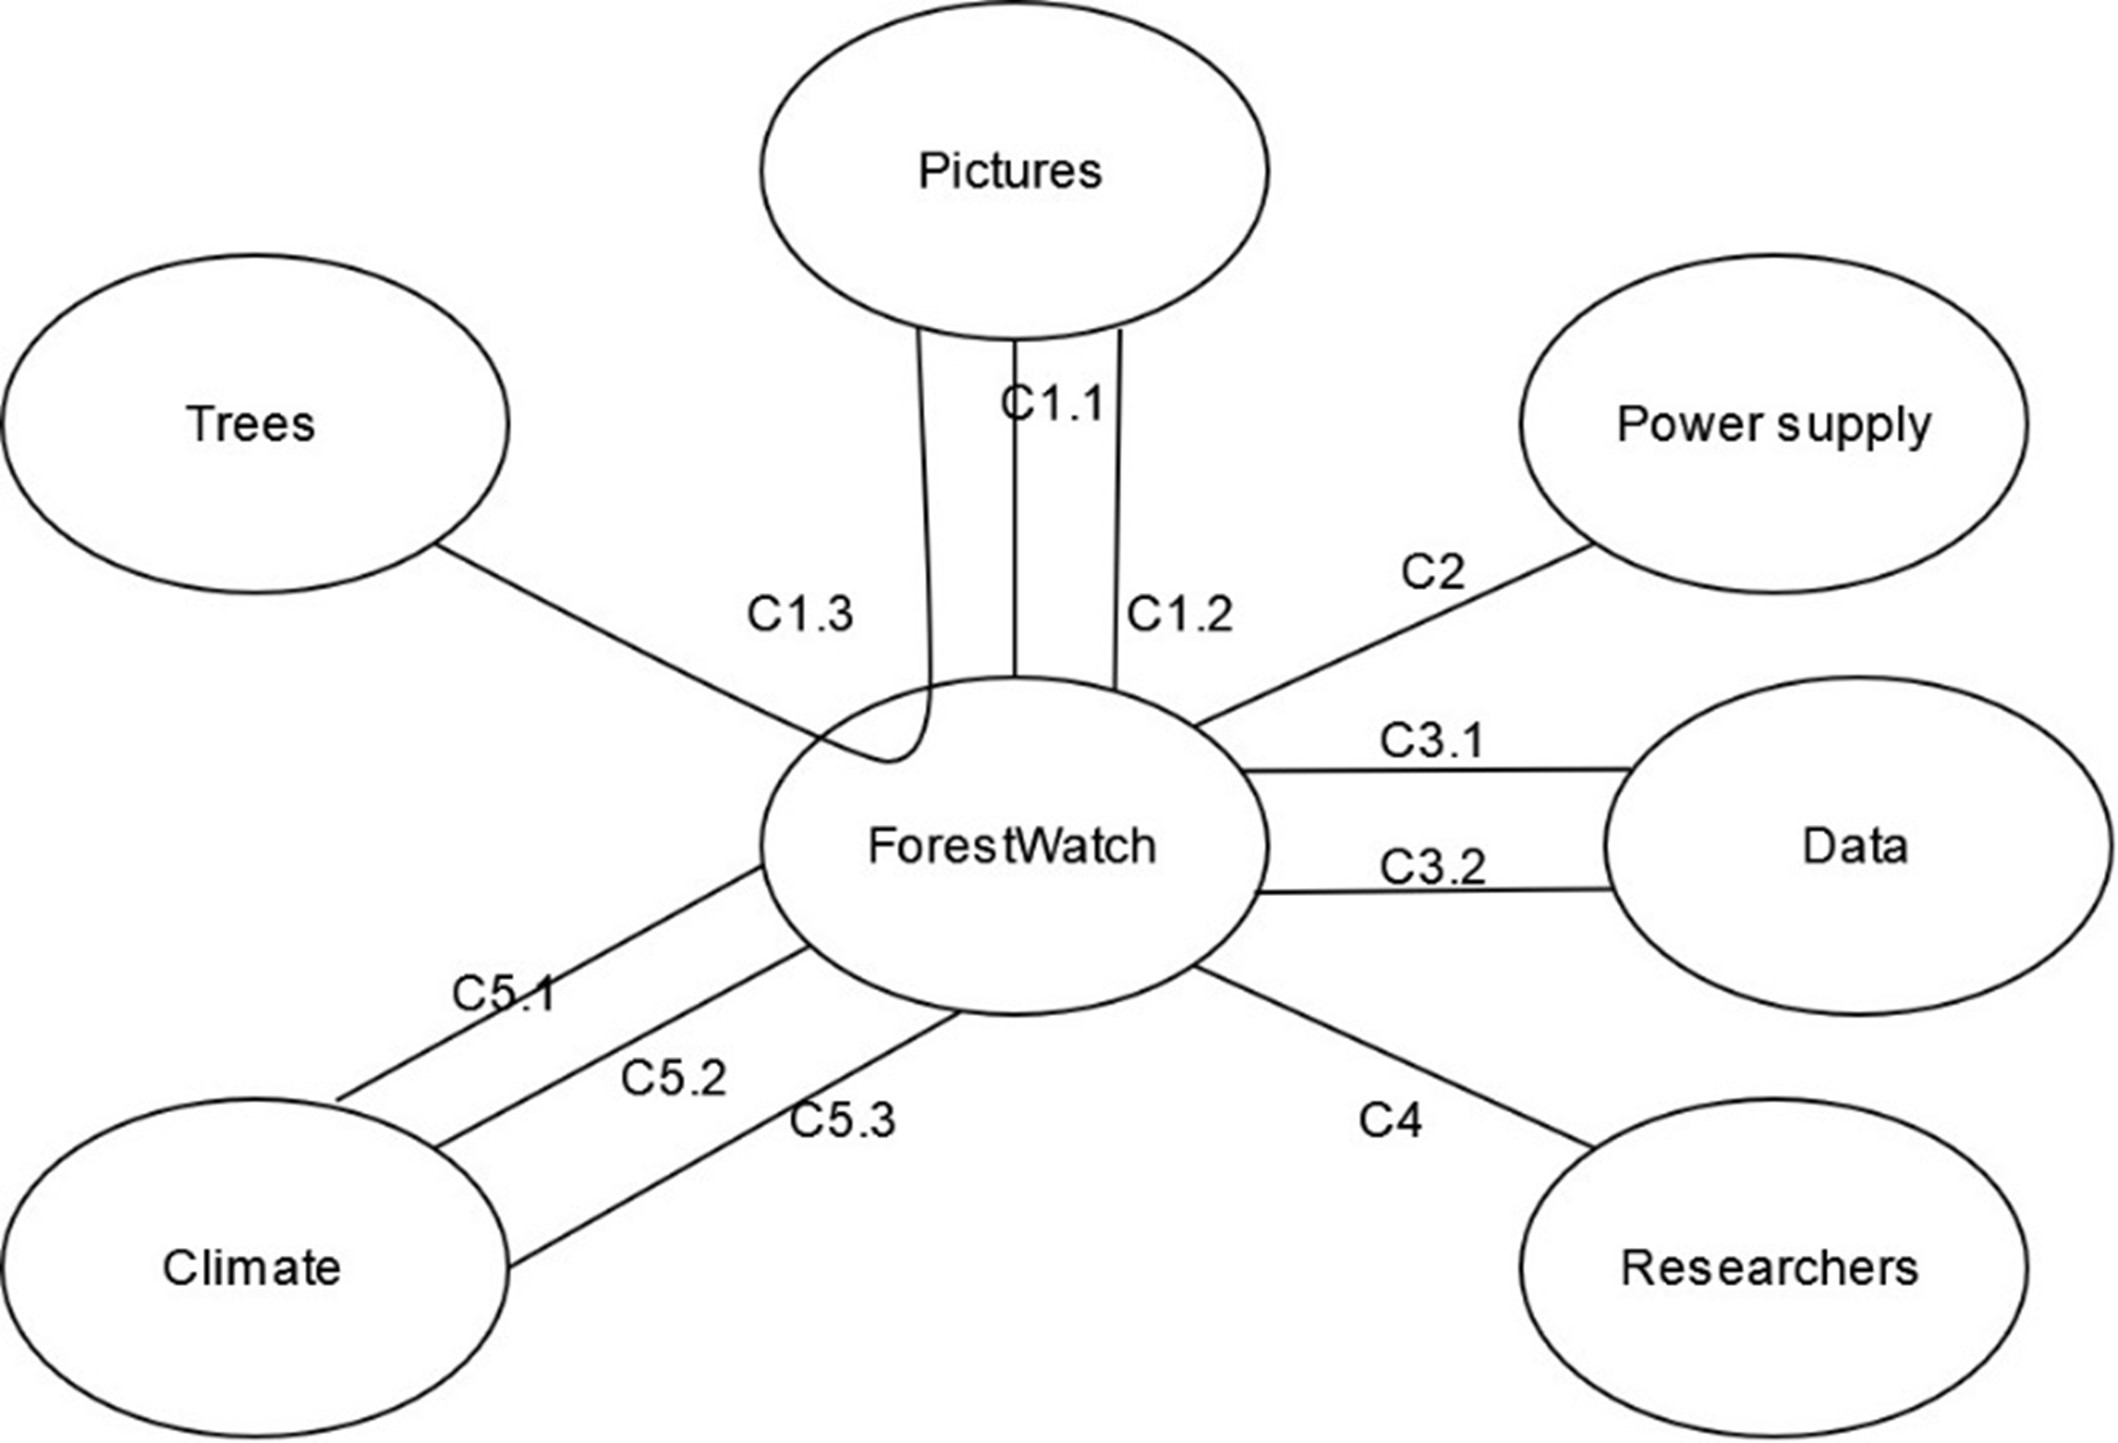
\includegraphics[width=0.8\textwidth]{\currfiledir/figures/technical_constraints.jpg}
    \caption{Graph presenting the different elements exercising constraints on the system.}
\end{figure}

\begin{itemize}[label=]
    \item C1.1: Calibrating internal camera.
    \item C1.2: Taking pictures twice a day.
    \item C1.3: Taking good quality pictures from 300 meters.
    \item C2: The system can stay autonomous for one year.
    \item C3.1: The system has 16 Go of space to store pictures.
    \item C3.2: The system has 16 Mo of space dedicated to log the information about the state of the system.
    \item C4: Transmitting data (temperature, remaining storage space and motions) over 10 kilometres.
    \item C5.1: Resisting to more than 90\% of humidity.
    \item C5.2: Resisting to temperatures from 20°C to 35°C.
    \item C5.3: Compliance with IP X4 norm or equivalent.
\end{itemize}
